\section[Diagonalisierung und Skalarprodukt]{Diagonalisierung, Bilinearformen, Skalarprodukt und Orthonormalbasen}
\Einleitung{Diese Woche ernten wir die Früchte unserer wochenlangen Vorarbeit: Wir sehen, dass die darstellende Matrix einiger Endomorphismen\footnote{Ein allerletztes Mal: Lineare Abbildungen eines Vektorraums in sich selbst.} bezüglich bestimmter Basen von $V$ eine Diagonalgestalt annimmt.\\
Diese bestimmten Basen setzen sich aus den Eigenvektoren des Endomorphismus zusammen. Wir betrachten also, unter welchen Bedingungen das möglich ist, und wechseln dann zum nächsten Thema:\\
Linearformen schnappen sich einzelne Vektoren und bilden sie auf Zahlen ab,\footnote{in diesem Zusammenhang hattet ihr den Dualraum kennengelernt}  während Bilinearformen sich jeweils zwei Vektoren schnappen und diese je auf eine Zahl abbilden. Diese Abbildungen müssen dabei u.a. linear sein. Unter bestimmten Umständen nennen wir eine Bilinearform auch (euklidisches\footnote{solange wir uns auf die reellen Zahlen $\mathbb{R}$ beziehen. Wir werden auch noch hermitesche Skalarprodukte kennenlernen, die für komplexe Vektorräume relevant sind.}) Skalarprodukt. Einen reellen Vektorraum mit einer solchen Abbildung bezeichnen wir dann als euklidisch, und wir sehen, dass sie sogar ausgezeichnete Basen (die Orthonormalbasen) haben.}

\subsection{Diagonalisierung von Endomorphismen}
\begin{Def}{Diagonalisierbarkeit}
Wir nennen einen Endomorphismus $F\in\End(V)$ \red{diagonalisierbar}, wenn eine Basis $B=(\bvec_1,...,\bvec_n)$ von $V$ existiert, bezüglich derer die darstellende Matrix $M_B(F)$ von $F$ \red{Diagonalgestalt} hat, d. h.
\begin{equation}
    M_B(F)=\diag(\lambda_1,\ldots,\lambda_n)=:\Matrix{\lambda_1&\cdots&\cdots&0\\
    \vdots&\lambda_2&&\vdots\\
    \vdots& & \ddots &\vdots\\
    0&\cdots&\cdots&\lambda_n},\quad\lambda_i\in\mathbb{K}\,\forall i
\end{equation}
\blue{Diese besondere Basis besteht aus den Eigenvektoren $\bvec_i$ von $F$ und die Diagonalelemente sind genau die Eigenwerte $\lambda_i$ dazu.}
\end{Def}
\blue{Um einen Endomorphismus zu diagonalisieren, müssen wir also die Eigenvektoren finden, und es muss genau $n=\dim V$ linear unabhängige Eigenvektoren geben, damit er diagonalisierbar ist. Letzteres ist auch die Aussage der folgenden Sätze:}
\begin{Satz}
{Satz}{Zerfall in Linearfaktoren}
Ist $F$ diagonalisierbar, so zerfällt das charakteristische Polynom $P_F(\lambda)$ in Linearfaktoren.
\end{Satz}
\blue{Das bedeutet, dass $P_F(\lambda)$ in der Form
\begin{equation*}
    P_F(\lambda)=\alpha\prod_{i=1}^n(\lambda-\lambda_i),\quad \alpha\in\mathbb{R}
\end{equation*}
geschrieben werden kann.\\
Da das charakteristische Polynom nicht von der Wahl der Basis abhängt, können wir es auch einfach mit der diagonalisierten Matrix berechnen:
\begin{equation*}
    P_F(\lambda)=\det(M_B(F)-\lambda\mathds{1}_n)=\prod_{i=1}^n(\lambda_i-\lambda).
\end{equation*}
Die Umkehrung gilt aber nur in bestimmten Fällen. Daher kann es auch wichtig sein, über welchem Körper euer Vektorraum definiert ist:\\
So zerfällt z. B. $P_F(\lambda)=(\lambda^2+1)=(\lambda+i)(\lambda-i)$ nur über $\mathbb{C}$ in Linearfaktoren, über $\mathbb{R}$ ist eine solche Zerlegung nicht möglich.}\\
Allerdings wissen wir noch nicht sicher, ob ein Endomorphismus diagonalisierbar ist, nur weil dessen charakteristisches Polynom in Linearfaktoren zerfällt. Entscheidend ist zudem die Dimension der zugehörigen Eigenräume, was in folgendem Satz festgehalten wird:
\begin{Satz}
{Satz}{Zur Diagonalisierbarkeit}
Für $F\in\End(V)$ (wobei $V$ endlichdimensional sei) gilt die folgende Äquivalenz:
\begin{itemize}
    \item $F$ ist diagonalisierbar.
    \item $P_F(\lambda)$ zerfällt in Linearfaktoren \underline{und} die geometrische und algebraische Vielfachheit stimmt für alle Eigenwerte überein, $n_{\lambda_i}=m_{\lambda_i}\,\forall \lambda_i$.
    \item $V$ ist die direkte Summe aus den Eigenräumen:\footnote{Dies ist eigentlich nur ein abstrakter Weg um zu sagen, dass die Vereinigung der Basisvektoren der Eigenräume eine Basis von $V$ bilden.} $V=\underset{\lambda\in\tx{EW}}{\bigoplus}V_\lambda$.
\end{itemize}
\end{Satz}
\blue{Jetzt seht ihr hoffentlich, weshalb wir uns letzte Woche die algebraische\footnote{Exponent des Eigenwertes im charakteristischen Polynom} und geometrische\footnote{Dimension des Eigenraums zum Eigenwert} Vielfachheit so genau angesehen haben.}
\begin{Satz}
{Kochrezept}{Diagonalisierung von Endomorphismen}
Um Endomorphismen zu diagonalisieren (oder zu testen, ob das überhaupt möglich ist), kann man auch nach folgendem Schema vorgehen:\\
Sei $(F:V\to V)\in\End(V)$ mit $\dim V=n$.
\begin{enumerate}
    \item (Ermittle die darstellende Matrix $A$ von $F$ bzgl. irgendeiner Basis\footnote{i. d. R. der kanonischen Basis}. Ist oft auch direkt gegeben.)
    \item Stelle das charakteristische Polynom auf: $P_A(\lambda)=\det(A-\lambda\mathds{1}_n)$.
    \item Ermittle die Nullstellen des charakteristischen Polynoms: $P_A(\lambda)=0$.\\
    Die ermittelten $\lambda_i$ sind die Eigenwerte.\\
    Zerfällt das charakteristische Polynom \textit{nicht} in Linearfaktoren, d. h. $\sum_{\lambda_i}m_{\lambda_i}<\dim V$, so ist $F$ nicht diagonalisierbar.
    \item Bestimme zu jedem $\lambda_i$ die Eigenvektoren $\bvec_{\lambda_i,j}$,\footnote{Dies können für einen Eigenwert $\lambda_i$ auch mehrere linear unabhängige sein, aber immer $\leq$ algebraische Vielfachheit des Eigenwerts.} indem $(A-\lambda_i\mathds{1}_n)\bvec_{\lambda_i,j}=\Vec{0}$ gelöst wird.
    \item Schreibe daraus die jeweiligen Eigenräume (als Span aus linear unabhängigen Eigenvektoren) auf.
    \item Ist die Summe der Dimensionen der Eigenräume $n$?
    \begin{enumerate}
        \item Wenn nein, so ist $F$ nicht diagonalisierbar.
        \item Wenn ja, so ist $F$ diagonalisierbar mit der darstellenden Matrix
        \begin{equation*}
            M_B(F)=\diag(\lambda_1,\ldots,\lambda_m)=\Matrix{\lambda_1&\cdots&\cdots&0\\
    \vdots&\lambda_2&&\vdots\\
    \vdots& & \ddots &\vdots\\
    0&\cdots&\cdots&\lambda_m}.
        \end{equation*}
        Hierbei tritt ein Eigenwert genau so oft auf, wie die Dimension des Eigenraumes ist.\footnote{Wenn zu $\lambda_i$ z. B. $n_{\lambda_i}=2$ ist, so tritt $\lambda_i$ zweimal auf der Diagonalen auf.}\\
        Die Eigenvektoren $\bvec_{\lambda_i,j}$ bilden dann genau die Basis $B=(\bvec_1,...,\bvec_n)$, bezüglich derer $F$ die Diagonalgestalt annimmt.
    \end{enumerate}
\end{enumerate}
\end{Satz}
Dieses Kochrezept wollen wir uns an folgendem Beispiel klar machen:
\begin{Beispiel}{Anwendung des Kochrezepts}
Sei $F:\mathbb{K}^3\to \mathbb{K}^2,\quad F(x,y,z)=\Matrix{x+3z\\y\\2x+z}$.\\
Ist $F$ über $\mathbb{R}$ bzw. über $\mathbb{C}$ diagonalisierbar?
\begin{enumerate}
    \item Bezüglich der kanonischen Basis $\hat{B}$ lesen wir ab:\footnote{Schaut euch einfach an, was $F$ mit den Einheitsvektoren macht, um die Einträge der Matrix zu bestimmen. Die erste Spalte ist das, was $F$ mit $\evec_1=\MatrixInline{1\\0\\0}$ macht usw.}
    \begin{equation*}
        A:=M_{\hat{B}}(F)=\Matrix{1&0&3\\0&1&0\\2&0&1}.
    \end{equation*}
    Wir sehen, dass $A\MatrixInline{x\\y\\z}=F(x,y,z)$ ist.
    \item Das charakteristische Polynom ist
    \begin{eqnarray*}
        P_A(\lambda)&=&\det\Matrix{1-\lambda&0&3\\0&1-\lambda&0\\2&0&1-\lambda}\\
        &\overset{\footnote{Regel von Sarrus}}{=}&(1-\lambda)^3-6+6\lambda\overset{\footnote{Binomischer Lehrsatz}}{=}1+3\lambda^2-3\lambda-\lambda^3-6+6\lambda\\
        &=&-\lambda^3+3\lambda^2+3\lambda-5.
    \end{eqnarray*}
    \item Wir raten die erste Nullstelle: $\lambda_1=1$. Mit Polynomdivision finden wir:
    \begin{equation*}
        P_F(\lambda):(\lambda-1)=-\lambda^2+2\lambda+5
    \end{equation*}
    Setzen wir dies gleich 0 und wenden nach Multiplikation mit $(-1)$ die $p$-$q$-Formel an, so finden wir
    \begin{equation*}
        \lambda_{2,3}=1\pm \sqrt{6},
    \end{equation*}
    es gilt also
    \begin{equation*}
        P_A(\lambda)=(\lambda-1)(\lambda-1+\sqrt{6})(\lambda-1-\sqrt{6}).
    \end{equation*}
    Das charakteristische Polynom zerfällt also in Linearfaktoren mit den jeweiligen algebraischen Vielfachheiten von 1.
    \item Wir suchen die Eigenvektoren zu den verschiedenen Eigenwerten, indem wir die Eigenwertgleichung $A\Vec{v}=\lambda \Vec{v}$ lösen:
    \begin{itemize}
        \item Zu $\lambda_1=1$:
        \begin{align*}
            &\MatrixInvertieren{1-1&0&3\\0&1-1&0\\2&0&1-1}{0\\0\\0}=\MatrixInvertieren{0&0&3\\0&0&0\\2&0&0}{0\\0\\0}\\
            &\implies 0x_2=0\implies x_2=t_1\in\mathbb{K},\,x_1=0=x_3.
        \end{align*}
        Also sehen wir: $\bvec_1=t_1\MatrixInline{0\\1\\0}$.
        \item Zu $\lambda_2=1-\sqrt{6}$:
        \begin{equation*}
            \MatrixInvertieren{\sqrt{6}&0&3\\0&\sqrt{6}&0\\2&0&\sqrt{6}}{0\\0\\0}\implies x_2=0,\, x_1=-\frac{\sqrt{6}}{2}x_3\implies x_3=t_2\in\mathbb{K}.
        \end{equation*}
        Also sehen wir: $\bvec_2=t_2\MatrixInline{-\sqrt{6}/2\\0\\1}$.
        \item Zu $\lambda_3=1+\sqrt{6}$:
        \begin{equation*}
            \MatrixInvertieren{-\sqrt{6}&0&3\\0&-\sqrt{6}&0\\2&0&-\sqrt{6}}{0\\0\\0}\implies x_2=0,\, x_1=\frac{\sqrt{6}}{2}x_3\implies x_3=t_3\in\mathbb{K}.
        \end{equation*}
        Also sehen wir: $\bvec_3=t_3\MatrixInline{\sqrt{6}/2\\0\\1}$.
        \item Die Eigenräume sind dann also
        \begin{align*}
            \lambda_1&=1:\quad V_1=\Spann{\MatrixInline{0\\1\\0}}\\
            \lambda_2&=1-\sqrt{6}:\quad V_1=\Spann{\MatrixInline{-\sqrt{6}/2\\0\\1}}\\
            \lambda_3&=1+\sqrt{6}:\quad V_1=\Spann{\MatrixInline{\sqrt{6}/2\\0\\1}}.
        \end{align*}
        Die geometrische Vielfachheit ist jeweils $n_{\lambda_i}=\dim V_{\lambda_i}=1=m_{\lambda_i}$.
        \item Für alle Eigenwerte ist $n_{\lambda_i}=m_{\lambda_i}$ und $\sum_{i=1}^3\dim V_{\lambda_i}=3=\dim(\mathbb{K}^3)$.\\
        Die diagonalisierte Matrix ist daher
        \begin{equation*}
            M_B(F)=\diag(1,1-\sqrt{6},1+\sqrt{6})=\Matrix{1&0&0\\0&1-\sqrt{6}&0\\0&0&1+\sqrt{6}}.
        \end{equation*}
        Die zugehörige Basis ist $B=\MengeDirekt{\MatrixInline{0\\1\\0},\MatrixInline{-\sqrt{6}\\0\\2},\MatrixInline{\sqrt{6}\\0\\2}}$.\\
        $F$ ist also über $\mathbb{R}$ und somit auch über $\mathbb{C}$ diagonalisierbar.
    \end{itemize}
\end{enumerate}
\blue{Anmerkung:\\
Tatsächlich gilt $M_B(F)=\varphi_B^{-1}M_{\hat{B}}(F)\varphi_B$:\footnote{Hierbei ist $\varphi_B$ die Basiswechselmatrix zwischen der kanonischen Basis und der Basis $B$, die wir bestimmen, indem wir einfach die Basisvektoren spaltenweise aufschreiben.}
\begin{center}
    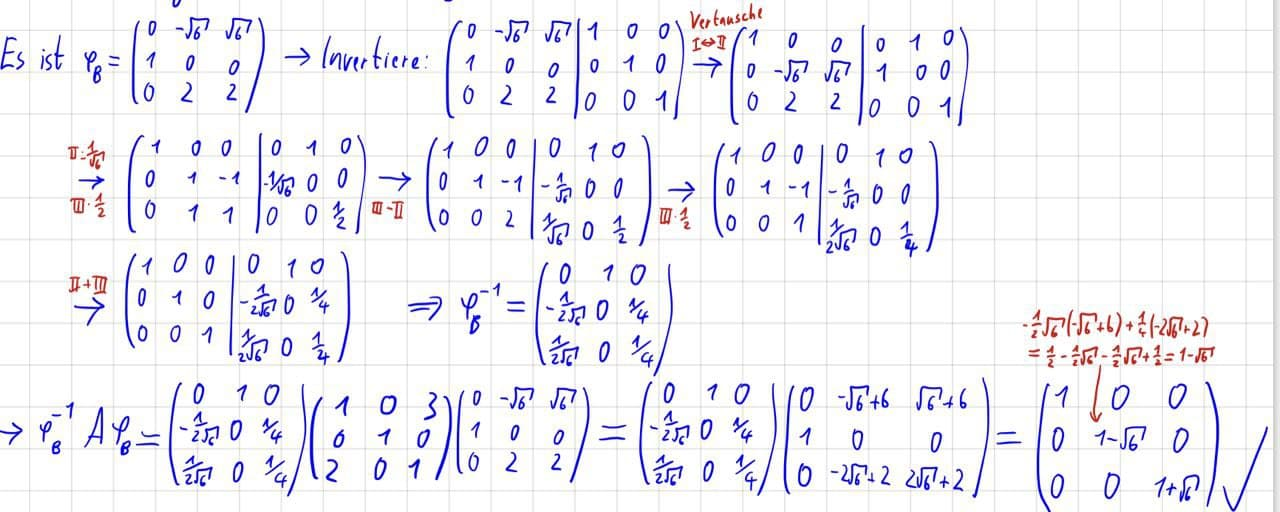
\includegraphics[width=.75\textwidth]{Dateien/03/03Diagonalisierung.jpg}
\end{center}}
\end{Beispiel}
\subsection{Längen- und Winkelmessungen mit Vektoren}
\blue{Unser nächstes Ziel ist nun, Längen, Abstände und Winkelbeziehungen zwischen Vektoren sinnvoll zu definieren. Wichtige Begriffe sind hierbei das Skalarprodukt, die Norm, Orthogonalität und die Cauchy-Schwarzsche Ungleichung.}


\subsubsection{Linearformen}
\begin{Wiederholung}
{Linearform}
Zunächst erinnern wir uns an den Begriff der \red{Linearform} aus MfP1:\\
Dies waren \underline{lineare Abbildungen}, die Elemente eines Vektorraumes $V$ über $\mathbb{K}$ in den Körper $\mathbb{K}$ abbilden, also $L\in L(V,\mathbb{K})$.\\
Die Menge aller solchen linearen Abbildungen wird \red{Dualraum} $V^*$ von $V$ genannt, also $V^*=\MengeDirekt{L:V\to\mathbb{K}}$.\\
Für endlichdimensionale Vektorräume $V$ mit $\dim V=n$ ist auch $\dim V^*=n$ und wir können die sog. \red{duale Basis} $B^*=(\bvec_1^*,\ldots,\bvec_n^*)$ zu einer Basis $B=(\bvec_1,\ldots,\bvec_n)$ von $V$ anhand folgender Forderung\footnote{die analog dazu ist, dass $\varphi_{B^*}\circ\varphi_B=\mathds{1}_n$ ist} definieren:
\begin{equation}
    \bvec_i^*(\bvec_j)=\delta_{ij}=\Cases{1&i=j\\0\,&i\neq j}.
\end{equation}
\blue{Zum Finden der dualen Basis kann man die Matrix aus Basisvektoren invertieren und dann die Zeilenvektoren als duale Basisvektoren ablesen.}\\
Die darstellende Matrix von Linearformen können wir uns als $1\times n$ Zeilenvektoren vorstellen.
\end{Wiederholung}
\begin{Beispiel}
{Linearform und darstellende Matrix über $\mathbb{R}$ (1/3)}
Wir betrachten den $\mathbb{R}^3$ mit der kanonischen Basis $\hat{B}=\MengeDirekt{\MatrixInline{1\\0\\0},\MatrixInline{0\\1\\0},\MatrixInline{0\\0\\1}}$. Die duale Basis wäre dann schlicht $\hat{B}^*=\MengeDirekt{\MatrixInline{1\\0\\0}^T,\MatrixInline{0\\1\\0}^T,\MatrixInline{0\\0\\1}^T}$, denn es gilt ja $\evec_i^*\evec_j=\delta_{ij}$.\\
Eine Linearform wäre z. B. die Abbildung $F:\mathbb{R}^3\to\mathbb{R},\, F(x,y,z)=2x-y+3z$. Diese hätte bzgl. $\hat{B}$ die folgende darstellende Matrix:
\begin{equation*}
    M_{\hat{B}}(F)=\Matrix{2&-1&3}\overset{\wedge}{=}2\evec_1^*-\evec_2^*+3\evec_3^*.
\end{equation*}
\end{Beispiel}
\begin{Beispiel}{Duale Basis im $\mathbb{C}^3$ (2/3)}
Sei  $B=\MengeDirekt{\MatrixInline{i\\0\\1},\MatrixInline{1\\1\\0},\MatrixInline{1\\1\\i}}$.\\
\Zz{Dies ist eine Basis von $\mathbb{C}^3$\footnote{Aufgefasst als Vektorraum über $\mathbb{C}$ - Als Vektorraum über $\mathbb{R}$ wären sechs Basisvektoren notwendig.} und die duale Basis ist\\ $B^*=\MengeDirekt{\MatrixInline{-i\\i\\0}^T,\MatrixInline{-1\\2\\i}^T,\MatrixInline{1\\-1\\-i}^T}$}
\Zb{$B$ ist eine Basis von $\mathbb{C}^3$, denn sie verfügt über drei linear unabhängige Vektoren, weil
\begin{equation*}
    \det \varphi_B=\det\Matrix{i&1&1\\0&1&1\\1&0&i}=i^2+1-1=-1\neq0.
\end{equation*}
Wir wollen nun die duale Basis finden. Wir suchen also $\varphi_{B^*}$, sodass $\varphi_{B^*}\circ \varphi_B=\mathds{1}_3$ ist. Es ist also nur die Inversion der Basismatrix $\varphi_B$ gefragt, und wir wissen ja, wie wir das machen:
\begin{align*}
    \MatrixInvertieren{i&1&1\\0&1&1\\1&0&i}{1&0&0\\0&1&0\\0&0&1}\overset{\I-\II,i\cdot\III}&{\longrightarrow}\MatrixInvertieren{i&0&0\\0&1&1\\i&0&-1}{1&-1&0\\0&1&0\\0&0&i}\\
    \overset{\III-\I,-i\cdot\I}&{\longrightarrow}\MatrixInvertieren{1&0&0\\0&1&1\\0&0&-1}{-i&i&0\\0&1&0\\-1&1&i}\\
    \overset{\II+\III,-1\cdot\III}&{\longrightarrow}\MatrixInvertieren{1&0&0\\0&1&0\\0&0&1}{-i&i&0\\-1&2&i\\1&-1&-i}.
\end{align*}
Wir lesen also ab: $\bvec_1^*=\Matrix{-i&i&0},\,\bvec_2^*=\Matrix{-1&2&i},\,\bvec_3^*=\Matrix{1&-1&-i}$.\\
Hierbei sind die $\bvec_i^*\in\Met(1,3,\mathbb{C})$ als lineare Abbildungen von $\mathbb{C}^3\to\mathbb{C}$ zu sehen.}\\
Wir betrachten nun die Abbildung $G:\mathbb{C}^3\to\mathbb{C},\, G(x,y,z)=x+y-iz$.\\
Wie sieht die darstellende Matrix dieser Abbildung bzgl. der Basis $B$ aus?\\
Wir nutzen die Gleichung $F(\vvec_j)=\sum_{i=1}^ma_{ij}\wvec_i,\,j=1,\ldots,n$ aus MfP1, um die darstellende Matrix zu bestimmen, wobei $v_j\in B$ und $\wvec_i\in B^*$ sind. Mit $V=\MengeDirekt{(1)}=:\MengeDirekt{\vvec_1}$ als Basis von $\mathbb{C}$ haben wir dann
\begin{align*}
    G(\bvec_1)&=i-i=0\overset{!}{=}a_{11}\vvec_1\\
    G(\bvec_2)&=1+1=2\overset{!}{=}a_{12}\vvec_1\\
    G(\bvec_3)&=1+1-i^2=3\overset{!}{=}a_{13}\vvec_1.
\end{align*}
Wir sehen also: $M_B^V(G)=\Matrix{0&2&3}$.\\
Diese Einträge könnten wir nun auch bzgl. der dualen Basis $B^*$ ausdrücken, aber das sparen wir uns.
\end{Beispiel}
\begin{Beispiel}
{Das Integral als Linearform (3/3)}
Für integrierbare Funktionen $R$\footnote{Mit $I$ bezeichnen wir für dieses Beispiel also den Raum der integrierbaren Funktionen auf $[a,b]$} ist das Integral $\int: I\to \mathbb{R},\,f(x)\mapsto\int_a^bf(x)dx$ eine Linearform.
\end{Beispiel}


\subsubsection{Multilinearformen und Eigenschaften von Bilinearformen}
Wir verallgemeinern nun das Konzept auf mehrere Elemente aus $V$, die linear auf ein Element des Körpers $\mathbb{K}$ abgebildet werden:
\begin{Def}
{Multilinearform}
Abbildungen $\mu: V^k\to\mathbb{K},\,(\vvec_1,\vvec_2,\ldots,\vvec_k)\mapsto\mu(\vvec_1,\ldots,\vvec_k)$ nennen wir \red{$k$-Linearform}, wenn $\mu$ in allen Argumenten linear\footnote{d. h. die beiden Bedingungen für Linearität, $F(\lambda \vvec+\wvec)=\lambda F(\vvec)+F(\wvec)$ in allen Argumenten erfüllt} ist.
\end{Def}
$k$-Linearformen mit $k>2$ werden uns für's Erste nicht mehr über den Weg laufen. Stattdessen nimmt die 2-Linearform eine wichtige Rolle ein:
\begin{Def}
{Bilinearform}
Für einen $\mathbb{K}$-Vektorraum $V$ nennen wir eine Abbildung\\
$\beta: V\times V\to \mathbb{K},\, (\vvec,\wvec)\mapsto\beta(\vvec,\wvec)$ \red{Bilinearform}, wenn sie linear in beiden Argumenten ist:\\
$\forall \vvec,\wvec,\zvec\in V$ und $\forall \lambda, \mu\in\mathbb{K}$ gilt dann
\begin{align*}
    &\beta(\lambda \vvec+\mu \wvec,\zvec)=\lambda\beta(\vvec,\zvec)+\mu \beta(\wvec,\zvec)\\
    &\beta(\vvec, \lambda \wvec+\mu \zvec)=\lambda\beta(\vvec,\wvec)+\mu\beta(\vvec,\zvec).
\end{align*}
\end{Def}
Bevor wir zu den Beispielen kommen, folgen noch ein paar wichtige Definitionen, um Bilinearformen zu klassifizieren:
\begin{Def}
{Symmetrie{,} Schiefsymmetrie und Entartung}
Wir nennen eine Bilinearform $\beta:V\times V\to \mathbb{K}$...
\begin{itemize}
    \item ...\red{symmetrisch} $\iff\beta(\vvec,\wvec)=\beta(\wvec,\vvec)\quad\forall \vvec,\wvec\in V$.
    \item ...\red{schiefsymmetrisch} $\iff\beta(\vvec,\wvec)=-\beta(\wvec,\vvec)\quad\forall \vvec,\wvec\in V$.
    \item ...\red{nicht entartet} $\iff$ Die Abbildung $V\to V^*,\,\vvec\mapsto \beta(\vvec,\cdot)$ ist injektiv\\
    $\quad\iff\beta(\vvec,\wvec)=0\quad\forall \wvec\in V$ nur wenn $\vvec=0$.
\end{itemize}
\blue{Mit der darstellenden Matrix werden wir gleich ein Werkzeug kennenlernen, mit dem man diese Eigenschaften schnell überblicken kann.}
\end{Def}
\blue{Tipp:\\
Wenn ihr zeigen wollt, dass eine symmetrische Abbildung eine Bilinearform ist, zeigt zuerst die Symmetrie.\\
Anschließend könnt ihr die Linearität im 1. Argument zeigen und für das 2. Argument einfach mit der Symmetrie argumentieren.}

\begin{Beispiel}
{Bilinearform auf dem $\mathbb{R}^3$}\label{03:beispBiFo}
Die Abbildung $\gamma:\mathbb{R}^3\times \mathbb{R}^3\to \mathbb{R}$ mit
\begin{equation*}
    \gamma(\vvec,\wvec)=3v_1w_1-v_2w_2+v_3w_3+2v_3w_1+2v_1w_3
\end{equation*}
ist eine symmetrische Bilinearform, denn\footnote{mit $\vvec=\MatrixInline{v_1\\v_2\\v_3}$ und $\wvec=\MatrixInline{w_1\\w_2\\w_3}$} $\gamma(\vvec,\wvec)=\gamma(\wvec,\vvec)$, sie ist also symmetrisch.\\
Wir zeigen nun die Linearität im 1. Argument: Für alle $\vvec,\wvec,\zvec\in\mathbb{R}^3,\,\lambda,\mu\in\mathbb{R}$ ist
\begin{align*}
    \gamma(\lambda v+\mu \wvec,\zvec)&=3(\lambda v_1+\mu w_1)z_1-(\lambda v_2+\mu w_2)z_2+(\lambda v_3+\mu w_3)z_3\\
    &\quad +2(\lambda v_3+\mu w_3)z_1+2(\lambda v_1+\mu w_1)z_3\\
    &=\lambda(3v_1z_1-v_2z_2+v_3z_3+2v_3z_1+2v_1z_3)\\
    &\quad+\mu(3w_1z_1-w_2z_2+w_3z_3+2w_3z_1+2w_1z_3)\\
    &=\lambda\gamma(\vvec,\zvec)+\mu\gamma(\wvec,\zvec).
\end{align*}
Aufgrund der Symmetrie ist $\gamma$ auch im 2. Argument linear.\\
Wir haben also gezeigt, dass $\gamma$ eine symmetrische Bilinearform ist.
\end{Beispiel}
\begin{Satz}
{Satz}{Bilinearformen haben eine darstellende Matrix}
Für $n$-dimensionale Vektorräume mit Basis $B=(\bvec_1,\ldots,\bvec_n)$ können wir der Bilinearform $\beta:V\times V\to \mathbb{K}$ eine \red{darstellende Matrix} bzgl. $B$ zuordnen, die eine $n\times n$-Matrix mit den Einträgen \underline{$\alpha_{ij}=\beta(\bvec_i,\bvec_j)$} ist.\\
\blue{Zum Finden der darstellenden Matrix müssen wir also nur gucken, was $\beta$ mit den Basisvektoren macht.}
\end{Satz}
\begin{Satz}{Satz}
{Aussagen über Bilinearformen}
Die darstellende Matrix $M_B(\beta)$ liefert uns einen schnellen Blick auf die Eigenschaften der Bilinearform:
\begin{itemize}
    \item Symmetrie $\iff M_B(\beta)=M_B(\beta)^T$, also z. B. $\MatrixInline{1&-2\\-2&-3}=\MatrixInline{1&-2\\-2&-3}^T$.
    \item Schiefsymmetrie $\iff M_B(\beta)=-M_B(\beta)^T$.
    \item Nicht-Entartung $\iff M_B(\beta)$ ist invertierbar $\iff\det M_B(\beta)\neq 0$.
\end{itemize}
\end{Satz}

\begin{Beispiel}
{Darstellende Matrix einer Bilinearform: Kanonische Basis (1/2)}
Wir wollen die darstellende Matrix der in \hyperref[03:beispBiFo]{Beispiel 3.5} definierten Bilinearform $\gamma$ mit
\begin{equation*}
    \gamma(\vvec,\wvec)=3v_1w_1-v_2w_2+v_3w_3+2v_3w_1+2v_1w_3
\end{equation*}
bzgl. der kanonischen Basis bestimmen:\\
Hierfür kann man mehr oder weniger ablesen: $\gamma(\evec_1,\evec_1)=3\cdot 1\cdot 1+0=3$ usw. Also ist
\begin{equation}
    A:=M_{\hat{B}}(\gamma)=\Matrix{3&0&2\\0&-1&0\\2&0&1}\implies A=A^T,
\end{equation}
$A$ ist also symmetrisch.\\
Ist $\gamma$ entartet?\\
Nein, denn $\det A\overset{\footnote{Sarrus}}{=}3(-1)1-2(-1)2=-3+4=1\neq0$.
\end{Beispiel}

\begin{Beispiel}
{Darstellende Matrix einer Bilinearform: Sonstige Basis (2/2)}
Nun wollen wir für $\gamma$ für die Basis $B=\MengeDirekt{\MatrixInline{1\\1\\0},\MatrixInline{0\\2\\2},\MatrixInline{-1\\0\\-1}}$ die darstellende Matrix bestimmen.\\
Hierfür müssen wir die einzelnen Einträge $\alpha_{ij}$ berechnen, indem wir die jeweiligen Basisvektoren $\bvec_i$ und $\bvec_j$ in $\gamma$ einsetzen:
\begin{align*}
    \alpha_{11}&=\gamma(\bvec_1,\bvec_1)=3\cdot 1\cdot -1\cdot 1+0\cdot 0+0=2\quad \alpha_{12}=0-2+0+0+4=4,\\
    \alpha_{13}&=-3+0+0+0-2=-5,\quad \alpha_{22}=-4+4+0=0,\quad \alpha_{23}=-2-4=-6,\\
    \alpha_{33}&=3-0+1+2+2=8,\quad \alpha_{21}=\alpha_{12}=4,\quad \alpha_{31}=\alpha_{13}=-5,\quad\alpha_{32}=-3
\end{align*}
Hierbei haben wir für die letzten Einträge die bekannte Symmetrie ausgenutzt. Wir sehen also:
\begin{equation*}
    A_2:=M_B(\gamma)=\Matrix{2&2&-5\\2&0&-6\\-5&-6&8}.
\end{equation*}
Ihr fragt euch vielleicht, wieso man sich den ganzen Aufwand macht und was man damit überhaupt \textit{darstellen} kann.\\
Mit der darstellenden Matrix können wir für $\gamma$ sehr schnell auswerten, was mit Vektoren bzgl. der Basis geschieht.\\
Als Beispiel betrachten wir $\vvec_1:=2\bvec_1+\bvec_3$ und $\vvec_2:=\bvec_2-\bvec_3$.\\
Verschiedene Wege führen nun zu $\gamma(\vvec_1,\vvec_2)$:
\begin{itemize}
    \item Zunächst können wir $\vvec_1$ und $\vvec_2$ bzgl. der kanonischen Basis darstellen:
    \begin{equation*}
        \vvec_1=2\Matrix{1\\1\\0}+3\Matrix{-1\\0\\-1}=-\evec_1+2\evec_2-3\evec_3,\quad \vvec_2=\Matrix{0\\2\\2}-\Matrix{-1\\0\\-1}=\evec_1+2\evec_2+3\evec_3.
    \end{equation*}
    Damit ist dann
    \begin{align*}
        \gamma(\vvec_1,\vvec_2)&=\Matrix{-1&2&-3}\Matrix{3&0&2\\0&-1&0\\2&0&1}\Matrix{1\\2\\3}=\Matrix{-1&2&-3}\Matrix{9\\-2\\5}\\
        &=-9-4-15=-28.
    \end{align*}
    Achtung: Im ersten Schritt haben wir $\vvec_1$ bzgl. der dualen Basis dargestellt, was im Falle der kanonischen Basis einfach das Transponieren bedeutet. Im Allgemeinen müsst ihr hier aber vorsichtig sein.
    \item Explizite Berechnung:
    \begin{equation*}
        \gamma(\vvec_1,\vvec_2)=3(-1)-2\cdot 2+(-3)3+2(-3)1+2(-1)3=-3-4-9-6-6=-28
    \end{equation*}
    \item Indem wir $\vvec_1$ bzgl. der dualen Basis darstellen, würden wir finden, dass
    \begin{equation*}
        \gamma(\vvec_1,\vvec_2)=\vvec_1^*\cdot A\cdot \vvec_2=-28
    \end{equation*}
    ist. Allerdings sparen wir uns an dieser Stelle das Finden der dualen Basis und das Darstellen von $\vvec_1$, ihr könnt es gern als Übung machen, als Überprüfung seht ihr ja das Ergebnis.
\end{itemize}
\end{Beispiel}

\subsubsection{Das Skalarprodukt als Spezialfall von Bilinearformen}
\begin{Def}
{Positive Definitheit}
Eine weitere Eigenschaft, die wir \underline{symmetrischen} Bilinearformen zuschreiben, ist die \red{positive Definitheit}, wir nennen $\beta:V\times V\to \mathbb{K}$ positiv definit, wenn
\begin{equation}
    \beta(\vvec,\vvec)>0 \quad \forall v\in V\tx{ mit } v\neq0.
\end{equation}
Wir schreiben ab jetzt $\beta(\vvec,\wvec)=:\BiFo{\vvec,\wvec}$ und meinen damit symmetrische Bilinearformen $\BiFo{\cdot,\cdot}:V\times V\to \mathbb{K}$.
\end{Def}

\begin{Def}
{(Euklidisches) Skalarprodukt}
Ein \red{euklidisches Skalarprodukt} auf $V$ ist eine \underline{positiv definite} \underline{symmetrische Bilinearform} $V\times V\to \mathbb{R}$ auf einem reellen Vektorraum $V$.
\end{Def}
\begin{Def}
{Euklidischer Vektorraum}
Ist auf einem \underline{reellen} Vektorraum ein Skalarprodukt definiert, nennen wir ihn \red{euklidisch}.
\end{Def}
\begin{Satz}
{Kochrezept}{Skalarprodukt zeigen}
Um zu zeigen, dass eine Abbildung $V\times V\to\mathbb{R}$ ein eukl. Skalarprodukt ist, müssen wir also zeigen:
\begin{enumerate}
    \item Positive Definitheit:\\
    $\BiFo{\vvec,\vvec}=0\implies \vvec=0\quad \vvec\in V$\\
    $v=0\implies \BiFo{\vvec,\vvec}=0$\\
    $\BiFo{\vvec,\vvec}>0\quad \forall \vvec\neq 0$.
    \item Symmetrie:\\
    $\BiFo{\vvec,\wvec}=\BiFo{\wvec,\vvec}\quad \forall \vvec,\wvec\in V$.
    \item Bilinearität:\\
    $\BiFo{\lambda \uvec+\vvec,\wvec}=\lambda\BiFo{\uvec,\wvec}+\BiFo{\vvec,\wvec}$.\\
    Die Linearität im zweiten Argument folgt dann aus der Symmetrie.
\end{enumerate}
\end{Satz}
\begin{Beispiel}
{Das kanonische Skalarprodukt}
Das kanonische Skalarprodukt im $\mathbb{R}^n$ ist definiert als\\
$\BiFo{\cdot,\cdot}:\mathbb{R}^n\times\mathbb{R}^n\to\mathbb{R},\quad \BiFo{\Vec{x},\Vec{y}}=\sum_{i=1}^nx_iy_i$.\\
Dieses sollten die meisten von euch bereits aus der Schule oder Physikvorlesungen kennen. Am besten überlegt ihr kurz, ob und warum hier alle geforderten Eigenschaften erfüllt sind.
\end{Beispiel}
Konzeptionell ist es für euch wahrscheinlich zunächst seltsam, dass nicht nur das euch bekannte kanonische Skalarprodukt existiert, sondern dass der Begriff eigentlich viel allgemeiner gefasst ist und das kanonische nur ein Spezialfall ist. Gewöhnt euch dran, das gleiche passiert nun mit den Definitionen von Längen von Vektoren (der Norm) und Abständen von Vektoren.

\subsubsection{Die Vermessung von Vektorräumen: Normen, Metriken, Winkel und Orthogonalität}
\begin{Def}
{Vom Skalarprodukt induzierte Norm}
In euklidischen Vektorräumen bezeichnen wir mit $\boxed{\Norm{\vvec}:=\sqrt{\BiFo{\vvec,\vvec}}}$ die \red{Länge} bzw. \red{Norm} eines Vektors.\\
\blue{Achtung:\\
Auch auf nicht euklidischen Vektorräumen\footnote{also jenen ohne Skalarprodukt} kann man eine Norm definieren!\footnote{Diese muss dann, ähnlich wie die Metrik oder das Skalarprodukt, bestimmte Eigenschaften erfüllen. Dazu später mehr.} Genau genommen ist diese Definition nur die \textit{vom Skalarprodukt induzierte} Norm.}
\end{Def}
Den folgenden Begriff hattet ihr im Zusammenhang mit der Betragsmetrik auf $\mathbb{R}$ bzw. $\mathbb{C}$ schon kennengelernt:
\begin{Wiederholung}
{Metrik}
Eine \red{Metrik} ist eine Abbildung auf einer Menge $X$ mit der Form $d:X\times X\rightarrow \mathbb{R}_+\cup \{0\}$ mit den Eigenschaften
\begin{eqnarray*}
\red{M1}: & d(x,y)\geq 0\text{ und } d(x,y)=0\Leftrightarrow x= y &\red{'positiv definit'}\\
\red{M2}: & d(x,y)=d(y, x) &\red{'symmetrisch'}\\
\red{M3}: & d(x,y)\leq d(x, z)+d(y,z) & \red{'Dreiecksungleichung'}.
\end{eqnarray*}
\end{Wiederholung}
\begin{Def}
{Durch das Skalarprodukt induzierte Metrik}
Mithilfe dieser Längendefinition können wir uns den \red{Abstand} zwischen zwei Punkten $\xvec,\yvec\in V$ definieren:
\begin{equation}
    \boxed{d(\xvec,\yvec)=\Norm{\xvec-\yvec}=\sqrt{\BiFo{\xvec-\yvec,\xvec-\yvec}}}.
\end{equation}
Da hier immer ein Skalarprodukt zugrunde liegt, nennt man diesen Abstandsbegriff auch die \red{vom Skalarprodukt induzierte Metrik}.\\
\blue{Achtung:\\
Ist auf einem Vektorraum nur eine Norm definiert, so reicht das auch aus und wir nennen $d(\xvec,\yvec)=\Norm{\xvec,\yvec}$ die \red{von der Norm induzierte Metrik}. Allerdings ist selbst eine Norm nicht notwendig, Metriken können auch einfach so definiert werden, solange sie die Metrikaxiome erfüllen.}
\end{Def}
\begin{Satz}
{Satz}{Cauchy-Schwarzsche Ungleichung}
Für alle $\vvec,\wvec$ in einem euklidischen Vektorraum gilt:
\begin{equation}
    \boxed{\Abs{\BiFo{\vvec,\wvec}}\leq\Norm{\vvec}\cdot\Norm{\wvec}},
\end{equation}
wobei Gleichheit genau bei linearer Abhängigkeit von $\vvec$ und $\wvec$ gilt.
\end{Satz}
\blue{Diese Ungleichung ist auch in der Physik super wichtig.}
\begin{Beispiel}
{Cauchy-Schwarz für das kanonische Skalarprodukt}
Bzgl. des kanonischen Skalarprodukts im $\mathbb{R}^n$ sieht das dann so aus:
\begin{equation*}
    \Abs{\BiFo{\xvec,\Vec{y}}}=\Abs{\sum_{i=1}^nx_iy_i}\leq\sqrt{\sum_{i=1}^nx_i^2}\sqrt{\sum_{j=1}^ny_j^2}=\sqrt{\BiFo{\xvec,\xvec}}\sqrt{\BiFo{\yvec,\yvec}}=\Norm{\xvec}\cdot \Norm{\yvec}.
\end{equation*}
\end{Beispiel}

\begin{Def}
{Winkel}
Für $\vvec,\wvec\in V\setminus\MengeDirekt{\Vec{0}}$ ist der Winkel zwischen $v$ und $w$ definiert als
\begin{equation}
    \angle(\vvec,\wvec):=\arccos\frac{\BiFo{\vvec,\wvec}}{\Norm{v}\cdot\Norm{w}}\in[0,\pi]
\end{equation}
\end{Def}
\begin{Def}
{Orthogonalität}
Bei einem Winkel von $\pi\overset{\wedge}{=}90^\circ$ nennen wir $\vvec$ und $\wvec$ \red{orthogonal}. In diesem Fall gilt
\begin{equation}
    \BiFo{\vvec,\wvec}=0
\end{equation}
\end{Def}
\begin{wrapfigure}{r}[0pt]{.15\textwidth}
 \vspace{-15pt}
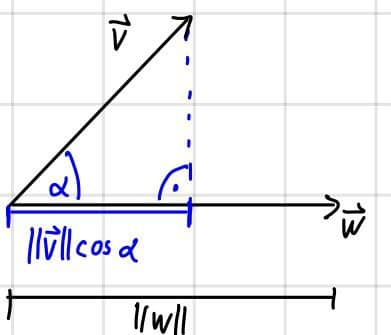
\includegraphics[width=.15\textwidth]{Dateien/03/03CauchySchwarz.jpg}
 \vspace{-5pt}
\end{wrapfigure}
\blue{Damit wird die Cauchy-Schwarzsche Ungleichung eventuell auch klarer:\\
Das Skalarprodukt projiziert den einen Vektor auf den anderen (daher der $\cos(\angle(\vvec,\wvec))$) und multipliziert die Beträge der Längen:\\
Die Projektion verschwindet genau bei Orthogonalität, bei linearer Abhängigkeit ist $\Abs{\BiFo{\vvec,\wvec}}=\Norm{\vvec}\cdot\Norm{\wvec}$.}


\subsubsection{Orthogonale Unterräume}
\blue{Anmerkung:\\
Dieses Kapitel ist unseres Erachtens unwichtig, aber gut für euer generelles Verständnis.}
\begin{Def}
{Orthogonaler Unterraum}
Zu jeder \underline{nicht entarteten} Bilinearform $\beta$ auf $V$\footnote{wobei $V$ ein endlichdimensionaler Vektorraum ist} und zu jedem Unterraum $U\subseteq V$ können wir uns den \red{zu $U$ $\beta$-orthogonalen Unterraum $U^{\perp_\beta}$} definieren.\\
Dieser beinhaltet alle Vektoren aus $V$, die bzgl. $\beta$ orthogonal zu Vektoren aus $U$ sind, d. h. $\BiFo{\uvec,\vvec}=0\,\forall \uvec\in U, \vvec\in U^{\perp_\beta}$. Als Menge aufgeschrieben ist also
\begin{equation*}
U^{\perp_\beta}:=\Menge{\vvec\in V}{\beta(\vvec,\uvec)=0\,\forall \uvec\in U}.
\end{equation*}
\end{Def}

Hierzu gibt es im Skript noch einige Sätze. Im folgenden sei $\beta$ eine nicht entartete Bilinearform, $V$ ein endlichdimensionaler Vektorraum und $U$ ein Unterraum.
\begin{Satz}{Satz}{Dimension des orthogonalen Raums}
Für die Dimension des orthogonalen Unteraums $U^{\perp_\beta}$ gilt
\begin{equation}
\dim U^{\perp_\beta}=\dim V- \dim U.
\end{equation}
\end{Satz}
\begin{Satz}
{Satz}{Komplementarität}
$U$ und $U^{\perp_\beta}$ sind genau dann komplementär, wenn $U\cap U^{\perp_\beta}=0$ ist.\\
\blue{In diesem Fall spannen also $U$ und $U^{\perp_\beta}$ zusammen den gesamten Vektorraum $V$ auf, was aus der linearen Unabhängigkeit der Vektoren aus $U$ und $U^{\perp_\beta}$ folgt.}
\end{Satz}
In euklidischen Vektorräumen ist dies stets der Fall.
\begin{Beispiel}
{Orthogonales Komplement}
Eine zweidimensionale Ebene ist ein Unterraum des $\mathbb{R}^3$. Das orthogonale Komplement besteht dann aus allen Vektoren, die orthogonal zu dieser Ebene sind, bzgl. des kanonischen Skalarproduktes also anschaulich senkrecht darauf stehen.
\end{Beispiel}


\Tipps{5}{
\begin{enumerate}
    \item
    \begin{enumerate}
        \item Erinnerung: Ein Polynom von mit Grad $\deg(P)=n$ könnt ihr so aufschreiben:
        \begin{equation*}
            P:\mathbb{C}\to\mathbb{C},\, P(z)=\sum_{k=1}^na_k z^k.
        \end{equation*}
        Was genau bedeutet die Achsensymmetrie bzgl. der reellen Achse? Anders gefragt: Was folgt für eine Nullstelle $z=a+bi$?
        \item Vielleicht war hier Aufgabenteil a) eine gute Vorbereitung. Wo taucht bei der Eigenwertbestimmung ein Polynom auf?\\
        Die Eigenwertgleichung inklusive der Definition der Eigenräume solltet ihr auch nochmal unter die Lupe nehmen.
    \end{enumerate}
    \item Hierfür lohnt es sich, noch einmal die Begriffe der algebraischen und geometrischen Vielfachheit nachzuschlagen. Welcher Satz setzt das in Zusammenhang mit der Diagonalisierbarkeit? Ansonsten ist das Rechnen nach Kochrezept. Salz nicht vergessen.\\
    Die Summe aller Eigenwerte sollte 2 ergeben.
    \item Für die darstellende Matrix betrachtet wieder die Wirkung von $\beta$ auf die Basisvektoren, die Einträge sind ja $\alpha_{ij}:=\beta(\bvec_i,\bvec_j)$, wobei $(\bvec_1,\bvec_2,\bvec_3,\bvec_4)=(1,x,x^2,x^3)$.\\
    Orientiert euch vielleicht an unseren Beispielen, um zu zeigen, dass dies eine symmetrische Bilinearform ist.
    \item \begin{enumerate}
        \item Schlagt noch einmal die Definitionen der Stetigkeit nach.
        \item Zeichnet euch das vielleicht kurz auf und nutzt a).
        \item Wie immer bei Skalarprodukten müsst ihr Symmetrie, Linearität in beiden Argumenten und positive Definitheit zeigen.\\
        Letzteres bedeutet, dass für $f\neq 0$-Funktionen (also $\exists x_0\in[0,1],$ sodass $f(x_0)\neq 0$) $\beta(f,f)>0$ ist.
    \end{enumerate}
\end{enumerate}
}